\casesection{Coriolis in a frictionless basin\label{case:corioliswithoutfriction}}


\paragraph*{Purpose}
The purpose of this testcase is to assess the ability of D-Flow FM to compute geophysical flows under influence of the Earth's rotation through the Coriolis force. In some cases, the computational results can be compared with (semi-)analytical solutions. This case comprises propagating waves in a rectangular, semi-closed basin for which a solution can be derived semi-analytically: the classical Taylor problem from 1921.

\paragraph*{Linked claims}
Claims that are related to the current test case are:
\begin{itemize}
\item \clrefnoh{cl:extforcingCoriolis}
\end{itemize}

\paragraph*{Approach}
A rectangular basin as given in \Fref{fig:wavesinbasinfricno} is adopted. The basin is closed at three edges and open at the boundary at $x = L$, with $L$ the length of the basin. For this setup, Taylor (1921) has figured out that the solution of the shallow water equations then yields the forcing Kelvin wave, a reflected Kelvin wave and an infinite number of so-called Poincar\'e waves. This solution can be derived semi-analytically using the \emph{collocation method}.

\begin{figure}[h!]
\begin{center}
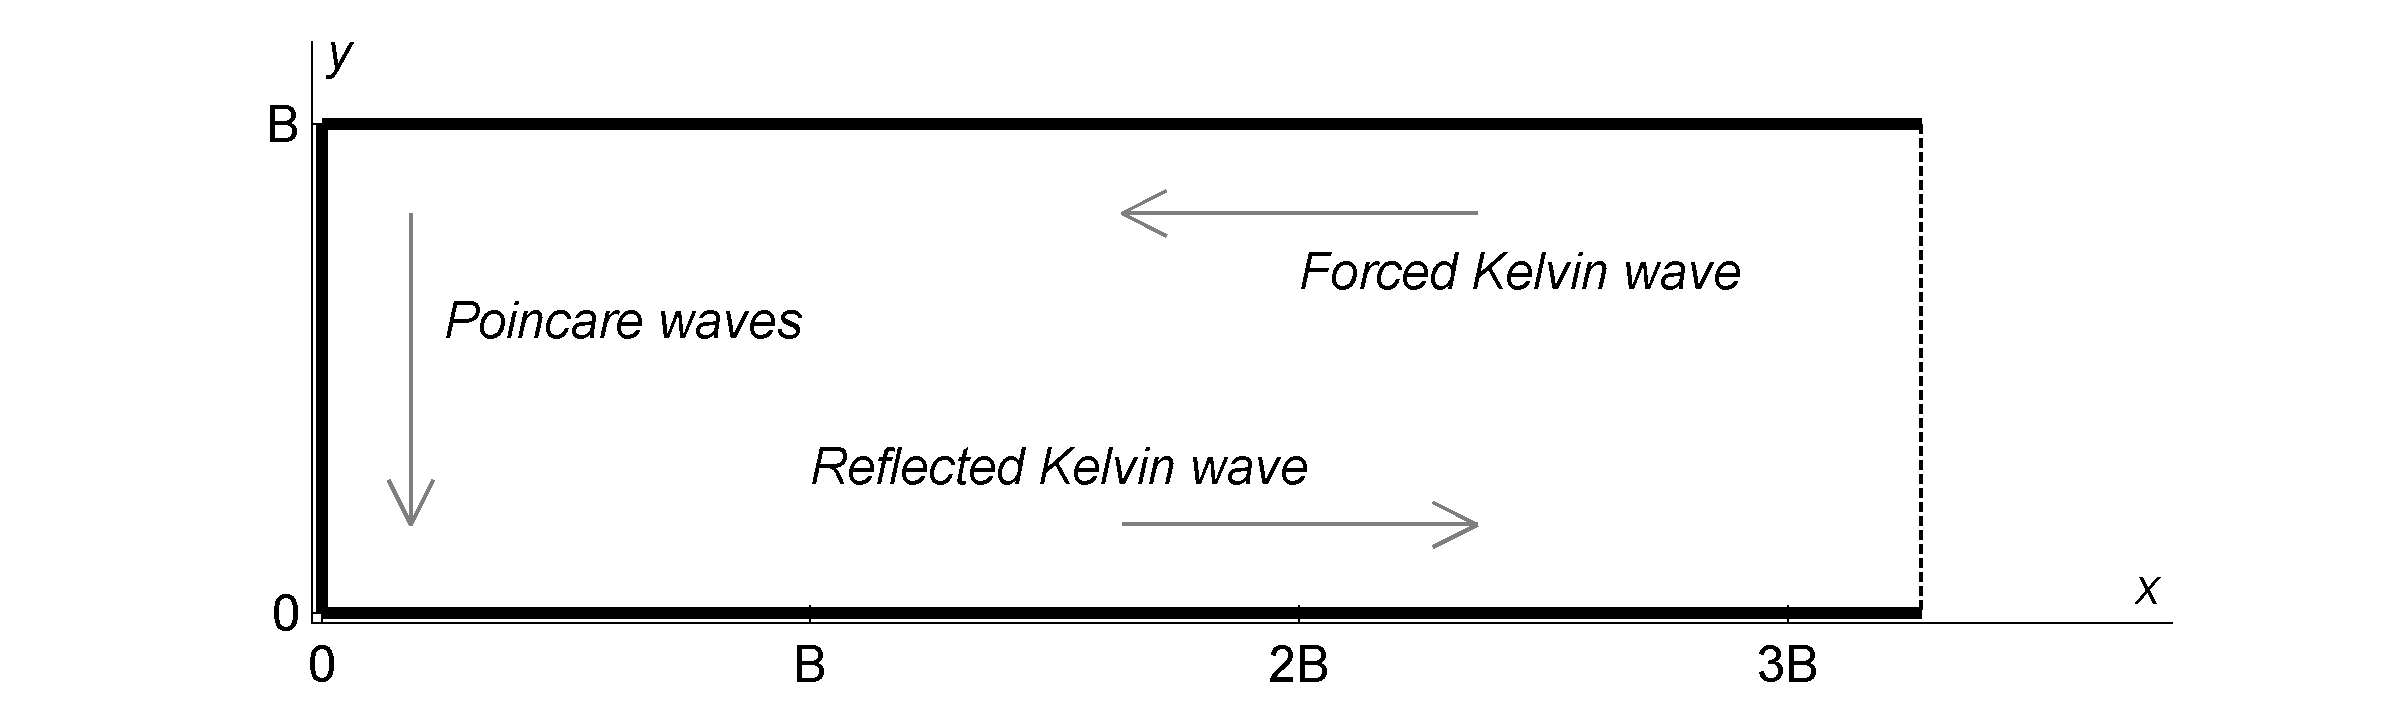
\includegraphics[width=1.0\columnwidth]{figures/basinplot.png}
\end{center}\caption{The classical Taylor problem: propagation of waves in a semi-closed basin of rectangular shape. \label{fig:wavesinbasinfricno}}
\end{figure}

To mimic the semi-analytical solution of Taylor, the water level elevation at the open boundary at $x=L$ is prescribed. This elevation, denoted by $\zeta$, is the sum of the incoming and outgoing Kelvin wave, based on the solution for an infinitely long channel bounded by sidewalls at $y = 0$ and $y = B$. These so-called pseudo-standing Kelvin waves are described by the following expression:
\begin{eqnarray}
\zeta(y) &=& \frac{2c}{g}U_0 \exp \left(-\frac{fB}{2c} \right) \cdot  \cosh \left(\frac{f}{c} \left(\frac{B}{2}-y \right) \right) \cdot \cos kx \cos \omega t   \\
         &+& \frac{2c}{g}U_0 \exp \left(-\frac{fB}{2c} \right) \cdot  \sinh \left(\frac{f}{c} \left(\frac{B}{2}-y \right) \right) \cdot \sin kx \sin \omega t 
\end{eqnarray}
in which $B$ is the width of the basin, $g$ the gravitational accelaration, $f$ the Coriolis parameter being $f = 2 \Omega \sin \varphi$, with $\Omega$ the Earth's rotation $2\pi/24/3600 = 7.2722\cdot10^{-5}$ rad/s and $\varphi$ the latitude, $c$ the phase speed of the forcing's wave equal to $\sqrt{gH}$, with $H$ the water depth. The parameters $k$ and $\omega$ are the wavenumber and wavefrequency, respectively, and $U_0$ is the forcing's amplitude.

The expression for the surface elevation $\zeta$ can be rewritten as:
\begin{eqnarray}
\zeta_{in}(y) = \frac{c}{g}U_0 \cdot &\exp \left(-\frac{fB}{c}\right) \cdot &\exp \left(+ \frac{fy}{c} \right) \cdot \left(\cos kx \cos \omega t - \sin kx \sin \omega t   \right) \\
\zeta_{out}(y) = \frac{c}{g}U_0 \cdot &  &\exp \left(-\frac{fy}{c} \right) \cdot \left(\cos kx \cos \omega t + \sin kx \sin \omega t   \right)
\end{eqnarray}
which enables a prescription of the boundary conditions by means of two signals with different amplitude and with a mutual phase difference equal to the phase difference between $\cos kx \cos \omega t - \sin kx \sin \omega t$ and $\cos kx \cos \omega t + \sin kx \sin \omega t$.


\paragraph*{Model description}
The computational domain is the rectangular basin as shown in \Fref{fig:wavesinbasinfricno}. The chosen input for the domain is as follows:
\begin{itemize}
\item length $L$ $\times$ width $B$ is 1800 $\times$ 550 km$^2$,
\item the water depth $H$ is equal to 80 m (and hence, the phase speed $c$ is determined),
\item the latitude $\varphi = 52 \degr$ (and hence, the Coriolis parameter $f$ is determined),
\item the forcing amplitude $U_0$ is chosen equal to $c/g$,
\item the waveperiod $T$ of the forcing wave is equal to 745 minutes (and hence, the wavefrequency $\omega$ is determined as $\omega = 2\pi/T$ as well as the wavenumber $k$, namely as $k= \omega / c = \omega / \sqrt{gH}$).
\end{itemize}
The friction is turned off; the horizontal eddy viscosity has the uniform value of 0 m$^2$/s. The sidewalls are impermeable, but frictionless (normal velocities equal zero). At $x = L$ the phase lag between $\zeta_{in}$ and $\zeta_{out}$ can be computed as $45.12\degr$.

Three computational grids are examined: 
\begin{enumerate}
\item a coarse Cartesian grid consisting of $72 \times 22$ cells of $25.0 \times 25.0$ km$^2$,
\item a fine Cartesian grid consisting of $144 \times 44$ cells of $12.5 \times 12.5$ km$^2$,
\item a triangular grid with a typical cell edge size comparable to the typical grid size of the fine Cartesian grid.
\end{enumerate}


\paragraph*{Results}
The results for each of the three grids are shown in \Fref{fig:kelvinfricno} in comparison with the semi-analytical solution. Maximum surface elevations are shown.

\begin{figure}[h!]
\begin{center}
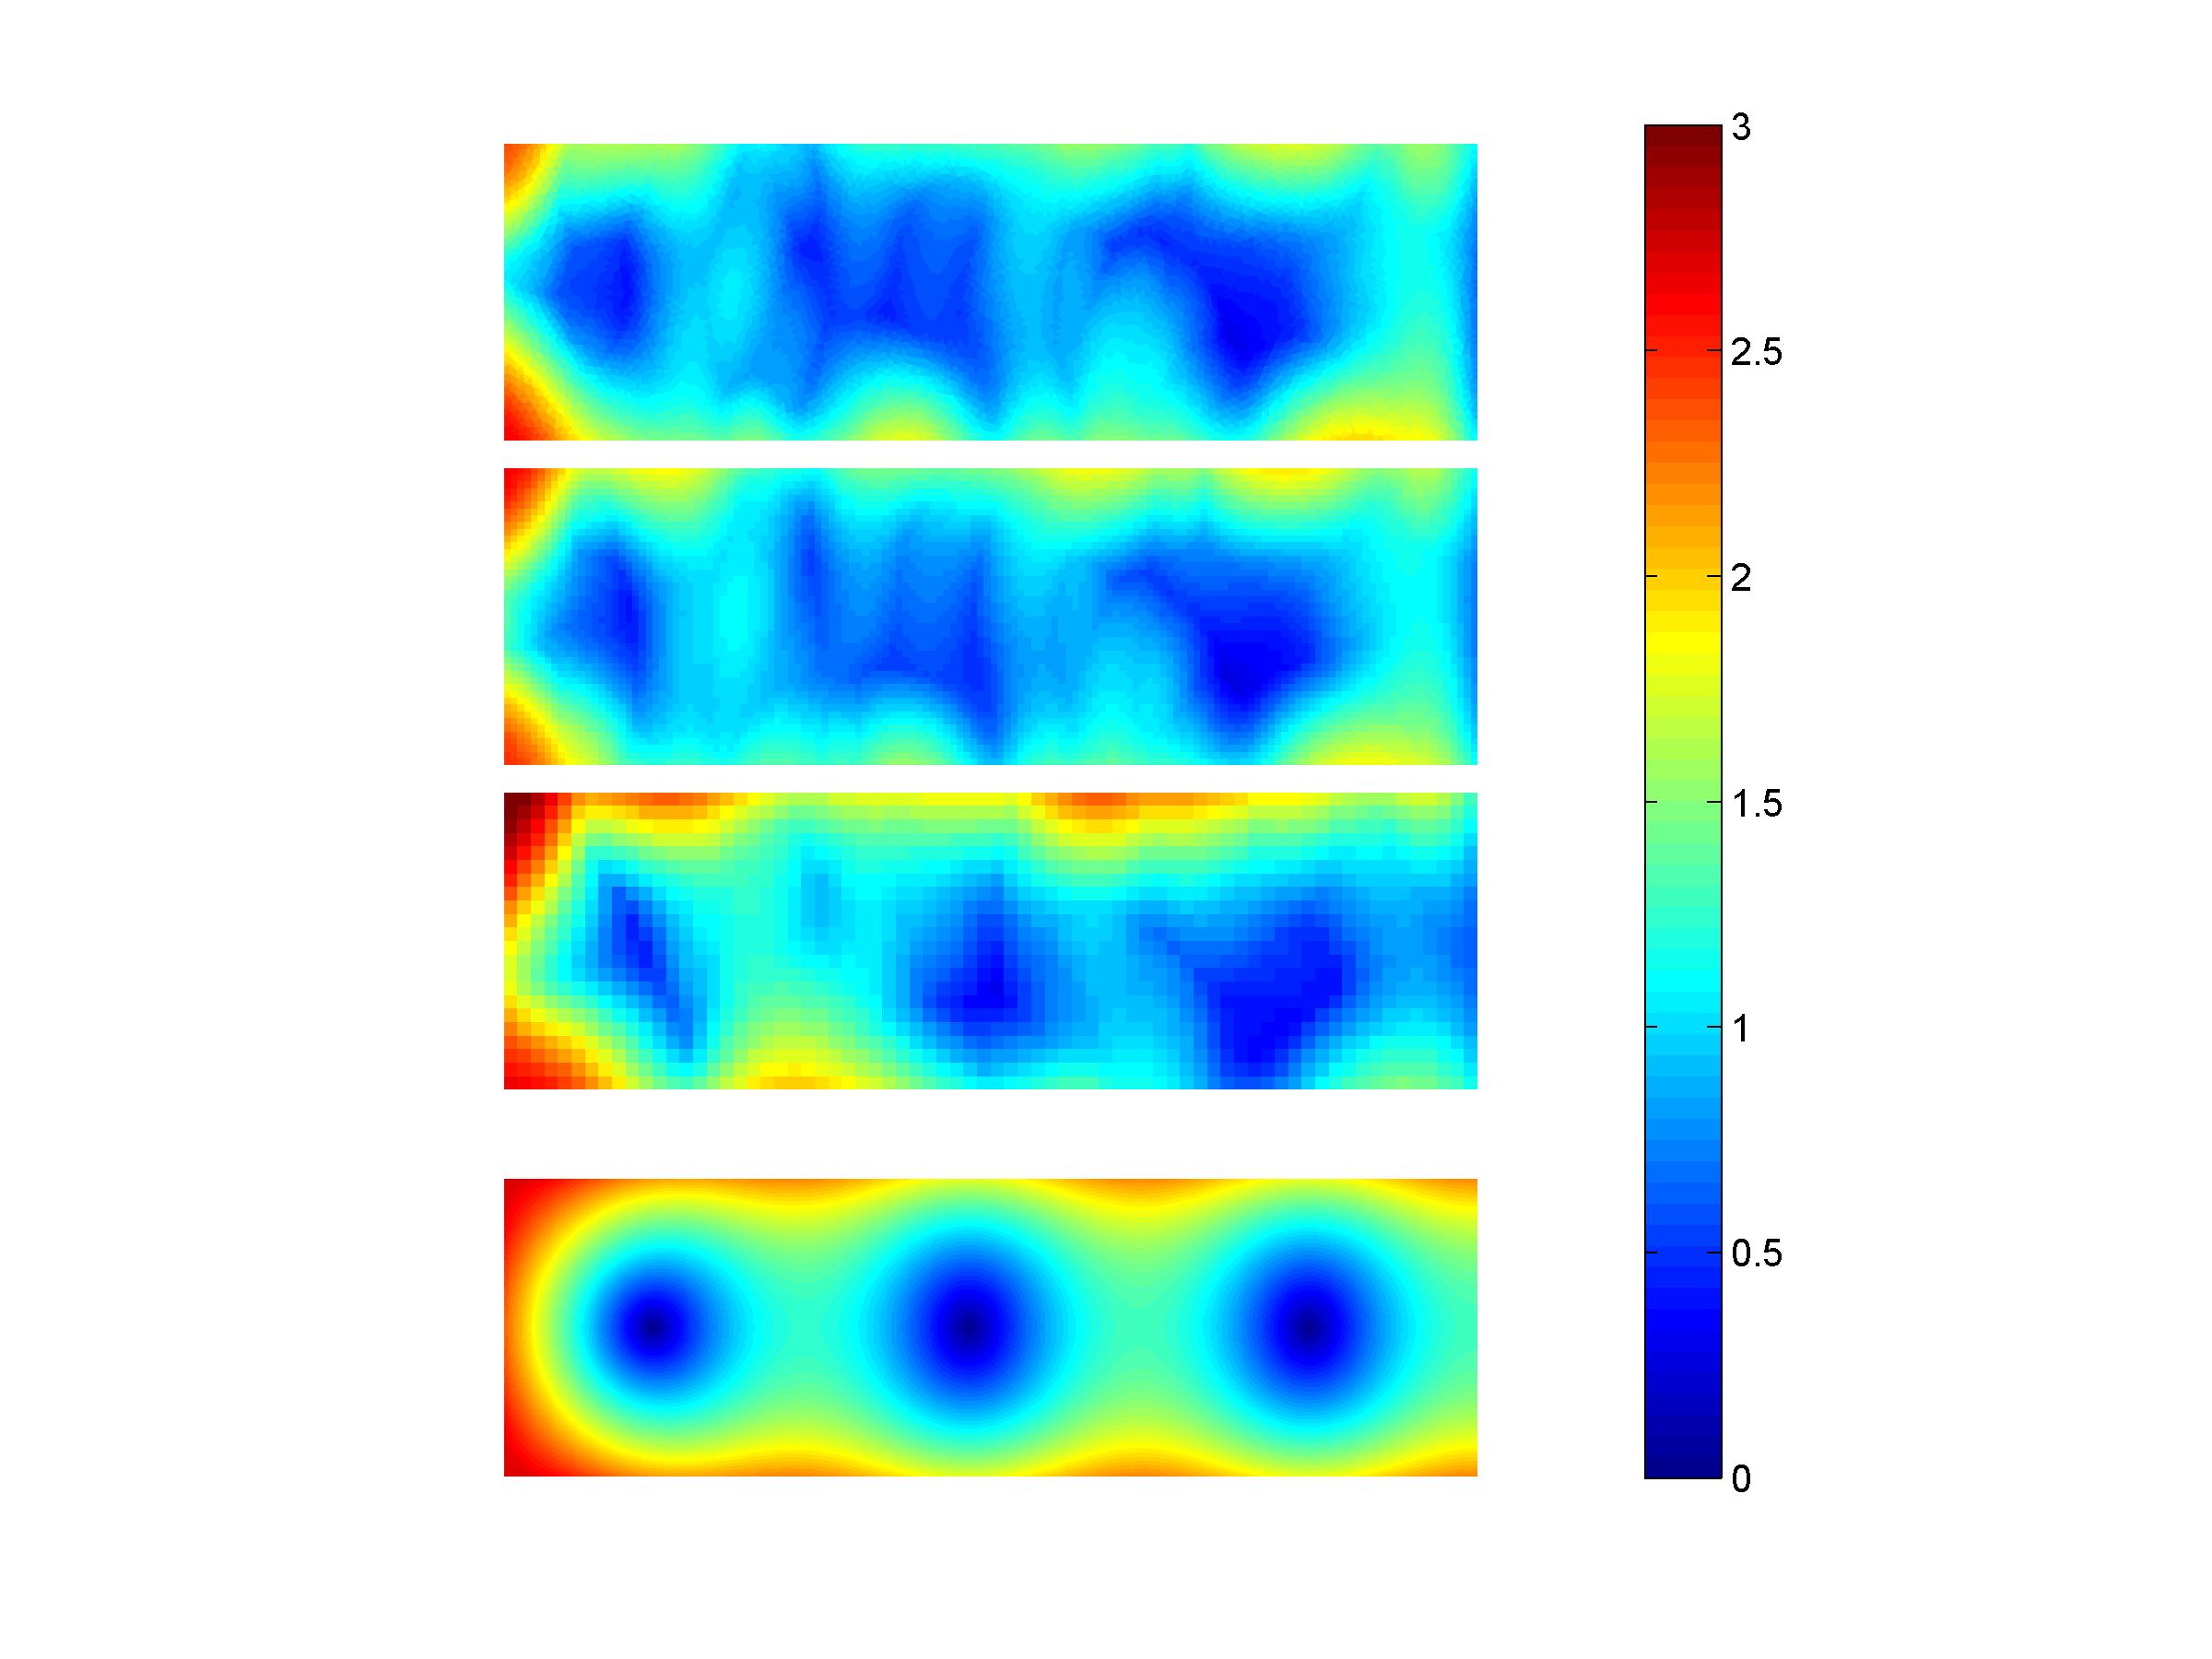
\includegraphics[width=1.0\columnwidth]{figures/basinnofriction.png}
\end{center}\caption{Semi-analytical solution (bottom panel) for the Coriolis test without friction. The upper three panels show the computational result from D-Flow FM on the triangular grid (upper panel), the fine Cartesian grid (second panel) and the coarse Cartesian grid (third panel). The colors span surface elevations from 0 m to 2.8 m. \label{fig:kelvinfricno}}
\end{figure}

The bottom panel (semi-analytical solution) shows a symmetric image of the absolute surface elevations. The solution, basically a superposition of the two Kelvin waves and a large number of Poincar\'e waves) consists of three amphidromic points. 

The computational results (the three top panels) show that D-Flow FM has difficulties in reproducing the amplitudes of the surface elevation. The location of the amphidromic points seems to agree with the semi-analytical solution. However, the image is diffuse. It should further be investigated what the explanation for this diffuse picture is. 




\paragraph*{Conclusion}
For geophysical flow under influence of the Coriolis force, but in the absence of friction and horizontal eddy viscosity, D-Flow FM experiences difficulties in reproducing the amplitudes of the surface elevation. The location of the amphidromic points seems to agree with the semi-analytical solution.



\paragraph*{Version}
This test has been carried out with version dflow-fm-x64-1.1.136.39235.


\paragraph*{Acknowledgement}
The writer is thankful to mr. Koen Berends for providing Matlab-scripts to compute the semi-analytical solution. These Matlab-scripts are based on: Roos, P.C., Velema, J.J., Hulscher, S.J.M.H., Stolk, A. (2011), An idealized model of tidal dynamics in the North Sea: resonance properties and response to large-scale changes, Ocean Dynamics, 61 (12), 2019-2035.


